\batchmode
\makeatletter
\def\input@path{{C:/Users/karlp/Documents/pragmatics/}}
\makeatother
\documentclass[12pt,english]{article}\usepackage[]{graphicx}\usepackage[]{color}
% maxwidth is the original width if it is less than linewidth
% otherwise use linewidth (to make sure the graphics do not exceed the margin)
\makeatletter
\def\maxwidth{ %
  \ifdim\Gin@nat@width>\linewidth
    \linewidth
  \else
    \Gin@nat@width
  \fi
}
\makeatother

\definecolor{fgcolor}{rgb}{0.345, 0.345, 0.345}
\newcommand{\hlnum}[1]{\textcolor[rgb]{0.686,0.059,0.569}{#1}}%
\newcommand{\hlstr}[1]{\textcolor[rgb]{0.192,0.494,0.8}{#1}}%
\newcommand{\hlcom}[1]{\textcolor[rgb]{0.678,0.584,0.686}{\textit{#1}}}%
\newcommand{\hlopt}[1]{\textcolor[rgb]{0,0,0}{#1}}%
\newcommand{\hlstd}[1]{\textcolor[rgb]{0.345,0.345,0.345}{#1}}%
\newcommand{\hlkwa}[1]{\textcolor[rgb]{0.161,0.373,0.58}{\textbf{#1}}}%
\newcommand{\hlkwb}[1]{\textcolor[rgb]{0.69,0.353,0.396}{#1}}%
\newcommand{\hlkwc}[1]{\textcolor[rgb]{0.333,0.667,0.333}{#1}}%
\newcommand{\hlkwd}[1]{\textcolor[rgb]{0.737,0.353,0.396}{\textbf{#1}}}%
\let\hlipl\hlkwb

\usepackage{framed}
\makeatletter
\newenvironment{kframe}{%
 \def\at@end@of@kframe{}%
 \ifinner\ifhmode%
  \def\at@end@of@kframe{\end{minipage}}%
  \begin{minipage}{\columnwidth}%
 \fi\fi%
 \def\FrameCommand##1{\hskip\@totalleftmargin \hskip-\fboxsep
 \colorbox{shadecolor}{##1}\hskip-\fboxsep
     % There is no \\@totalrightmargin, so:
     \hskip-\linewidth \hskip-\@totalleftmargin \hskip\columnwidth}%
 \MakeFramed {\advance\hsize-\width
   \@totalleftmargin\z@ \linewidth\hsize
   \@setminipage}}%
 {\par\unskip\endMakeFramed%
 \at@end@of@kframe}
\makeatother

\definecolor{shadecolor}{rgb}{.97, .97, .97}
\definecolor{messagecolor}{rgb}{0, 0, 0}
\definecolor{warningcolor}{rgb}{1, 0, 1}
\definecolor{errorcolor}{rgb}{1, 0, 0}
\newenvironment{knitrout}{}{} % an empty environment to be redefined in TeX

\usepackage{alltt}
\usepackage[T1]{fontenc}
\usepackage[latin9]{inputenc}
\usepackage{babel}
\usepackage[unicode=true]
 {hyperref}

\makeatletter
%%%%%%%%%%%%%%%%%%%%%%%%%%%%%% Textclass specific LaTeX commands.
\newcommand{\lyxaddress}[1]{
	\par {\raggedright #1
	\vspace{1.4em}
	\noindent\par}
}
\newenvironment{lyxcode}
	{\par\begin{list}{}{
		\setlength{\rightmargin}{\leftmargin}
		\setlength{\listparindent}{0pt}% needed for AMS classes
		\raggedright
		\setlength{\itemsep}{0pt}
		\setlength{\parsep}{0pt}
		\normalfont\ttfamily}%
	 \item[]}
	{\end{list}}

%%%%%%%%%%%%%%%%%%%%%%%%%%%%%% User specified LaTeX commands.
\usepackage{wrapfig}

\makeatother

\usepackage[bibstyle=authoryear,citestyle=chicago-authordate]{biblatex}
\addbibresource{0C__Users_karlp_Documents_pragmatics_pme.bib}
\IfFileExists{upquote.sty}{\usepackage{upquote}}{}
\begin{document}
\title{The Pragmatics of Private Markets Investing}
\author{Karl Polen}
\maketitle

\lyxaddress{Karl Polen is Chief Investment Officer at Arizona State Retirement
System\\karlp@azasrs.gov (for official communication with ASRS only)
\\karl.polen@gmail.com (for all other communication)}

\begin{abstract}
The author shares perspectives and lessons learned from four decades
experience in private markets investing.\\\\Key Takeaways:\\\\1.
Private markets investing is business investing and you need to focus
on the quality of the business approach in creating strategic advantage
in the markets served.\\\\2. Private markets investing is a hiring
decision and you need to assess the quality of the organization under
consideration for a strategy. Management should be expected to demonstrate
an ability to not just remain healthy, but grow and improve through
the tenure of your relationship with them.\\\\3. Managing cost of
fees is important, bot not sufficient to ensure success. Alignment
of interest across a range of outcomes, not just the upside, should
be given paramount importance in partnership structuring.
\end{abstract}
\pagebreak

In this paper I share perspectives about investing in private markets
developed during thirty years of private sector experience followed
by ten years in an institutional environment.\footnote{I have worked for the Arizona State Retirement System for the last
ten years, initially as Head of Private Markets Investing and as CIO
for the last 4 years. However, this work and the views it expresses
are my own. The policies of ASRS are set in accordance with its governance
policy and may be different from what is stated here. Any information
about ASRS is drawn from public information readily available on its
website. }These views incorporate a framework for investment decision making
and underwriting of strategies and firms. The process for assessing
strategies and firms is unavoidably qualitative and subjective. However,
I also present some analytical methods that I think are useful in
support of the decision process. 

Institutional investors have adopted the use of private markets strategies
in their portfolios at a rapidly increasing rate in recent decades.
The markets themselves have grown commensurately to multi-trillion
size. As the number of listed companies has declined, private markets
have become difficult to ignore. This paper does not, however, attempt
to justify the decision to invest in these markets or develop an approach
to incorporating them in a strategic asset allocation analytical framework.
It starts, instead, from a standpoint that those decisions have already
been made. 

When asked to explain the underwriting process for private markets
investing, I use the metaphor of a three legged stool. One leg each
for strategy, organization and track record. By strategy, I refer
to business strategy. What market are you addressing; what is your
competitive advantage and how do you think you will add value? As
a critical step in the process, we assess the health of the asset
management organization. Do they have the organizational depth and
skills to implement the target strategy? Have they created a culture
that will allow them to continue to grow and improve over the life
of the investment? We examine track record as confirmatory evidence
on the first two questions. Track record alone is a weak indicator
of likely future success. Finally, we consider the terms of an investment
partnership as to the appropriateness of the costs associated with
it and the reliability of the alignment of interest of the investor
and investment manager. 

\section*{STRATEGY}

As investors we learn we learn about strategy in the context of strategic
asset allocation; i.e. the proportion of assets allocated to risks
and associated premia related to equities, rates, credit, real estate
and so forth. These decisions are the most important determinant of
outcomes, at least after the fact. As important as this is, we are
using the word ``strategy'' in a different way. We are referring
to business strategy.

You can think of business strategy as the opposite of luck. It answers
the question ``how do we earn the profits we make.'' You earn them
because somebody values what you do and you do it well. Strategy endures.
Luck doesn't.

The history of private markets institutional investing goes back to
the 1980s and 1990s. In those days, mere liquidity was a strategy.
When the market suffered dislocations, for example in the RTC crisis
of the early 90s, private capital seized on opportunities that were
wildly mispriced. The RTC saw its mission as rapidly resolving failed
S\&Ls and they auctioned the assets individually and in pools to a
market that simply was not organized to absorb the volume of assets
delivered. 

The extraordinary returns earned during these times attracted additional
capital and a private capital industry has organized itself globally
with trillions of investment capacity. Private capital is now deeply
embedded in the structure of capital markets and an effective competitor
to public markets. It used to be that once a company reached a billion
or so in enterprise value, its only option to raise capital for growth
was in public markets. Following various crises of the last thirty
years, regulation of public companies and the increasing presence
of activist shareholders has increased the cost of going public and
reduced the attractiveness of it. In the meantime, the availability
of private capital and the competitiveness of private markets with
multiple firms bidding on deals has made it feasible and efficient
to finance firms to mid-cap and even large-cap range outside public
markets. This is a self-reinforcing cycle leading to continued growth
in private capital as investors seek access to these opportunities. 

In this context, liquidity and savvyness about discerning value and
opportunity are still needed but no longer sufficient. The sheer size
of private markets ensures competitive bidding for pretty much anything
that comes to market. In order to continue to earn excess returns,
the best private capital firms have invested in their firms to create
ever deeper expertise in the markets they address. They use this expertise
to create strategic advantage to generate or gain access to deals
and to formulate and execute business strategy for companies or properties
owned. This trend also drove firms to specialize. For all but the
very largest firms, there was a need to select which markets they
want to address in order to build teams to accomplish their objectives.

Private equity strategies can broadly be categorized as ``growth''
or ``value''. In growth approaches, your goal is to accelerate the
top line while optimizing operations to drive down unit costs enhancing
profitability or creating a path to it. In value strategies, you rationalize
operations in order to harvest cash flow. Practically any market offers
opportunities to build businesses and make money. The question for
the investor is whether the team you are evaluating is well prepared
to tackle the issues presented by the strategy they are pursuing.
In order to add value, the skills required will go well beyond financial
deal-making skills. In private equity, operations teams are critical.
If you are going to actually achieve ``synergy'' benefits when combining
two firms, you need to support the management teams in successfully
completing the necessary integration. Specialized industry expertise
is often essential, whether it's marketing and logistics expertise
for consumer brands or geologists and engineers who can evaluate ``quality
of rocks'' in oil and gas ventures. 

On the other hand, real estate delivers value to consumers through
design. Real estate design is the province of architects and urban
planners and the best firms incorporate them on their team. These
professionals are experts in consumer preference and craft a strategy
for building design responsive to location and environmental context
that creates a strategic advantage in fulfilling its commercial purpose.
Time and time again, we see well designed and operated buildings maintaining
high occupancy and earning premium rents in markets and neighborhoods
that otherwise would be regarded as highly competitive. Employment
trends, the tastes of millenials and impacts of technology are rapidly
changing what constitutes good design and risks of obsolescence in
real estate are high. Value strategies of investing in older buildings
at discount prices need to be evaluated carefully. Unlike other investment
categories where scale is usually paramount, the fundamental attractiveness
of real estate as an investment category is enhanced by the intensely
local nature of markets creating the opportunity for competitive advantage
and pricing power at relatively small scale. 

Credit strategies achieve their success through their access to deal
pipeline and discipline and diligence in deciding whether or not to
make a loan. Credit firms must have sourcing operation with extensive
relationships across the industry they serve. Lending decision require
deep expertise in credit analysis including industry coverage teams.
Once the loan is made, the die is largely cast. Nevertheless, active
monitoring is extremely important. Rapid action in addressing a deteriorating
credit can improve recovery rates. 

The final test of strategy is consumer-centeredness. We started out
by saying understanding strategy is similar to a firm grasp of the
answer to how a firm earns its profits. If it's lucky or exploitative,
it won't be sustainable. Firms have multiple constituencies and as
firms mature, they evolve in how they embrace their responsibilities.
For asset management firms, the first order customer is the asset
owner which has entrusted them with a portion of their capital for
management. The issues here are pretty straight-forward -- the asset
owner wants its money turned into more money together with some niceties
like being kept informed on how things are going along the way. More
to come on this when we discuss terms in a later section. 

To distinguish themselves, firms must serve a broader customer set.
Private equity firms serve the management teams of the companies they
own. A software industry investor adds value if it has an internal
consulting team with expertise in software development and marketing.
Such a firm becomes a preferred partner getting a last look in auctions
or even having the chance to buy businesses ``off market''. A middle
market credit firm adds value through its reputation for reliably
closing and fair dealing when conditions evolve for better or worse.
Such a firm can achieve premium pricing and hold firm on other terms
and covenants. 

Additionally, these relationships create access to deal flow. A firm
must demonstrate an ability to actually deploy capital, timely, in
the amount raised and consistent with the parameters of the promised
strategy. I am not put off by a firm's aspiration to grow and, realistically,
that is a goal for any firm of quality. However, an asset manager
should be prepared to demonstrate that their strategy is scalable
within the bounds of their fund raising aspirations, without drift
or deterioration in underwriting standards. 

Every firm has a critical internal customer set in the people who
work there. This is the topic of the next section.

\section*{ORGANIZATION}

Once you select strategies to pursue, you need to hire teams to implement
them. Private markets investing concerns itself principally with this
hiring decision. Though we analyze prior investments, it isn't the
same as securities analysis. When Warren Buffet drinks a Coca Cola
and reads their financial statements and decides he likes it, he then
can buy the stock and Coca Cola is what he gets. You can analyze the
prior track record of a private equity firm all you want, but you
don't get those deals. What you are evaluating is whether they have
created a culture and process that adds value and assessing whether
you think it is likely they will repeat that success.

You will start evaluating an organization simply by looking at the
size and composition of the team. Is it big enough and does it contain
the technical specialties necessary to implement the planned strategy.
A relevant statistic is firm assets under management divided by employee
headcount. From that information, you can calculate an estimate of
the recurring revenue per employee. The revenue should be high enough
to support the team allowing for continued growth and advancement.

Firm culture will be critical in the success of the firm and its investments.
One of the biggest challenges for a private markets investor is dealing
with situations where a firm deteriorates because of internal conflict,
shifts in focus or unplanned transitions. These situations typically
lead to poor investment results and if you can screen out firms at
risk for these outcomes, you will enhance your investment results.
Founder leadership style establishes and guides the culture. In building
a firm founders make a series of increasingly selfless decisions.
The first decision is to found the firm in the first place. The founders
have a fire in their belly to pursue something reflecting their unique
take on strategy and build something which is their own. This first
``at bat'' is critical -- if you don't have enough early success
to attract capital and talent, the firm never really gets off the
ground. As the firm progresses, the founders are then faced with the
task of transitioning from deal culture to firm culture. 

One of the fun things about being an investor in private markets is
the opportunity to meet many founders and observe how they manage
this journey. The best managers de-emphasize the personalities of
the founders in order to build the culture of the firm. Leaders in
this style see leadership as service and as an antonym to authority.
They build a culture reflecting a philosophy and discipline of business
practice and then trust the culture. Decisions and responsibility
are increasingly entrusted to the team as their skills and experience
grow. The founders don't hold themselves out as final decision makers.
Instead they monitor that appropriate discipline was observed in making
the decision and that feedback loops are present to appropriately
measure the outcome of the decision and learn from those outcomes.
Teamwork is emphasized. Every individual understands her role and
does not let down her colleagues with substandard, incomplete or tardy
work. People learn to trust each other in the integrity and professionalism
of their work. Leadership in this context serves the firm, the employees
and the culture. The leaders accept financial rewards only after taking
care of the team first. They are quick to credit the team for their
work.

Compensation and employment terms are important. This is where the
rubber hits the road. While it may be the case that employees will
be loyal to firms that create a rich employment experience full of
challenge, team comraderie and joy from shared experience of success,
this only goes so far and the firm will deteriorate if the riches
created are not properly shared. Persons in authority who accept rewards
for themselves without first taking care of their teams are creating
an intrinsically toxic environment. As the firm evolves, it will develop
formalized and for more senior personnel contractual arrangements
for sharing profit. Careers are emphasized and career conversations
about what this job means to each person occur regularly. The uniqueness
of individuals is a source of strength for the culture. Succession
planning and ownership of the asset management firm must be addressed
well in advance of founder retirement both to protect investors from
adverse consequences of unplanned transitions and to complete the
bond with the next generation of managers who will succeed the founders. 

The capital of an asset management firm is human capital. Founders
who make the short term sacrifice of building a high quality culture
that exists beyond them and will endure after them achieve more for
themselves and the markets they serve than those with a narrower view
of self interest.

Assessing these things is difficult. In my own case, I use a thought
experiment and ask myself if a firm is a place I would want my adult
children to work. Will they be continuously challenged with projects
and duties of increasing complexity as their skills grow? Will they
receive regular candid feedback and will they receive financial rewards
commensurate with the value of their work? Will they advance in a
career path suited to them providing opportunities for technical excellence
or the chance lead a team or a business line? Will the culture, however
demanding, avoid hazing rituals and allow them to grow as individuals
with interests and relationships beyond work? If it's a workplace
where you'd be proud and happy for your children to be associated
with it, then it has a decent chance of surviving and thriving.

\section*{TRACK RECORD}

Why do we look at track record? Luck and randomness are everywhere
and just because a firm has done well, it is far from certain it will
continue to do so. In public markets, there is some evidence that
strategies that have recently done well will deteriorate. In private
markets, the evidence for persistence of performance is, at best,
equivocal.

We understand all that, but care about track record anyway. We care
about it because it is the one unfudgeable and unspinnable piece of
evidence we have that might help us assess whether the firm has created
a quality culture and is pursuing a robust strategy. Track record
is evidence of talent and one hopes that talent will be sustained
and grow with experience and maturity in the context of a high quality
firm. What follows is an explanation for calculating performance metrics
for private equity style investments.



\subsection*{Traditional Methods of Performance Measurement}

Time weighted returns are the standard methodology for evaluating
and comparing investment performance in liquid markets. They are not
appropriate for PE investments which are typically in the form of
limited partnership interests where the financial sponsor has the
right to control the amount and timing of capital called in to the
partnership resulting in an ever changing amount of capital deployed. 

The traditional performance metrics for private equity are TVPI and
IRR. TVPI is \textquotedbl total value as a percent of invested\textquotedbl{}
and is simply the ratio of value received to investment. IRR refers,
of course, to internal rate of return. These traditional measures
collectively give a good sense of the performance of a particular
PE investment and allow you to compare private equity investments
to each other. Data services tracking private equity use a combination
of these metrics to rank performance in \textquotedbl quartiles\textquotedbl .
They customarily group funds to control for market context in \textquotedbl vintages\textquotedbl{}
based on the year the partnership began investing. So, a 2006 vintage
fund which invested across the global financial crisis and earned
a 10\% IRR might be a top quartile performer for that vintage, while
the same IRR might be below average for a 2010 vintage.

\subsection*{Public Market Equivalent methods }

Controlling for market context by vintage is useful but still crude
because there is a lot of variability of patterns of calling and returning
capital from fund to fund. A good method to compare private market
IRRs with public markets is what is needed. Steve Kaplan and Antoinette
Schoar formulated a method for calculating private equity performance
as a \textquotedbl public market equivalent\textquotedbl{} which
we will refer to as KSPME \parencite{Kaplan2005}. KSPME is calculated
as ratio of benefits to costs and a value greater than 1 indicates
performance above the opportunity cost benchmark. The calculation
is illustrated in the following formulas.

The required data are a time series of capital calls $C_t$, a time
series distributions $D_t$, a final value at time $n$ of $V_n$
and a time series of dividend adjusted market indices $M_t$. You
calculate a future value factor as the ratio of the market index at
time $n$ divided by the index at prior times $t$ as follows:

$$FV_t=\frac{M_n}{M_t}$$

You then multiply (pair-wise for each of the values) the future value
factor times calls and distributions 

$$C_{FV}=C_t * FV_t$$ ; $$D_{FV} = D_t * FV_t$$ 

You now have what you need to calculate

$$KSPME = \frac{\Sigma D_{FV} + V_n}{\Sigma C_{FV}}$$ 

KSPME is a wealth measure reflecting how much extra money you have
by investing in the private equity fund compared to an alternative
public markets investment.

Gredil, Griffiths and Stucke have proposed an additional metric, called
\textquotedbl Direct Alpha\textquotedbl , which converts KSPME to
annual rate \parencite{Gredil2014}. KSPME tells you how much extra
money you made and Direct Alpha tells the annual rate at which you
made it. Direct Alpha is calculated as the IRR of a time series constructed
by combining the future value adjusted calls (as negative numbers),
distributions and the final value. So, it uses exactly the same data
as KSPME but with different calculations to reduce the data to a single
measurement. 

$$Direct Alpha = \log{(1+IRR(-C_{FV},D_{FV},V_n))}$$

If you have an IRR of a private equity investment $IRR_{PE}$ calculated
as a discrete annual return, you can then calculate an $IRR_M$ that
you would have earned by investing in a market index with the same
timing of investments and withdrawals as the calls and distributions
of the private equity investment. 

$$\log{(1+IRR_M)} = \log{(1+IRR_{PE})} - DirectAlpha$$

KSPME and Direct Alpha supplement the traditional private equity performance
measurements with methods that allow you to compare the private returns
to public returns. In effect, these methods accurately measure the
opportunity cost of public market investments foregone with the allocation
to private markets. PME methods are not a magic bullet, but they are
very useful. Prior to these methods, it was difficult to benchmark
performance. PME methods provide a rigorous tool for assessing performance
relative to market which is an essential starting point for assessing
the quality of a firm and its strategies.\footnote{A detailed explanation with code and sample data demonstrating how
to perform PME analysis and other calculations described in this article
is found at \href{https://github.com/karlpolen/pragmatics}{https://github.com/karlpolen/pragmatics}}

\subsection*{Consideration of skewness}

One last topic on performance assessment deserves mention. As is well
known, stock market returns are skewed with a few outliers contributing
disproportionately to performance. Hank Bessembinder has shown that
only 4\% of stocks have contributed substantially all the outperformance
of the stock market since the great depression \parencite{Bessembinder2019}.We'd
like to see a similar positive outlier type of skewness in our private
markets investments. The data sets are too small in private markets
for any pretension of fancy statistics. I prefer something I call
a ``slugging percentage'' which is simply the percentage of deals
that have returned 3X or more of the initial investment. We then compare
that to the percentage of deals that have lost money and if it's comfortably
larger, we have evidence of the sort of skewness we are looking for.
In the next section, we will analyze the effect of incentive compensation
on the skewness of net returns and you will see that positively skewed
gross returns are needed to balance things out for the investor.
\begin{lyxcode}
\end{lyxcode}

\section*{COST AND PARTNERSHIP TERMS}

Private equity structures are complicated and difficult to analyze.
We present here some approaches to analyze general partner compensation
in real estate and private equity partnerships. Real estate and private
equity investments are typically owned in a partnership which includes
a general partner (the \textquotedbl sponsor\textquotedbl ) and
limited partners (\textquotedbl investors\textquotedbl ). The sponsor
organizes the investment, recruits the investors and manages the assets.
The general partner is typically compensated with an asset management
fee and an incentive fee.

The asset management fee is usually stated as a percent per annum
of assets under management. This can be either as a percent of \textquotedbl commited\textquotedbl{}
capital or \textquotedbl invested\textquotedbl{} capital. In the
former case, the fee is earned based on the amount the investors commit
from the inception of the partnership without regard to when the capital
is called. If the asset management fee is based on invested capital,
then the fee is calculated only on capital which has been called. 

The incentive fee (\textquotedbl carry\textquotedbl ) is typically
stated as a percent of profits. Profits are normally defined as the
gross profits of the investments after returning partnership expenses
including the asset management fee. Usually, a hurdle rate of return
must be achieved before sharing begins. So, a typical deal might be
stated as \textquotedbl 20\% carry over an 8\% pref with a 50\% catchup\textquotedbl .
This means that the investor has to earn at least an 8\% return after
fund level costs before the sponsor earns any carry. Above an 8\%
return, the sponsor gets half the profit (i.e. the catchup is 50\%)
until the ratio of profit split is 20\% to sponsor. Thereafter, the
profits are split 80\% to the investors and 20\% to the sponsor. Incentive
fees of 20\% over an 8\% hurdle are nearly universal in private equity.
But the catchup is negotiable, with somewhere in the 50\% to 100\%
range being typical. 

Figure 1 shows the fee at various gross returns for this structure.
Figure 2 shows the share going to sponsor and investor in this structure
with a 2\% asset management fee. 





\begin{figure}[h]
\emph{Analysis of private equity ``20 over 8 with 50\% catch up''} 

\begin{minipage}[t]{0.45\columnwidth}%
\begin{knitrout}
\definecolor{shadecolor}{rgb}{0.969, 0.969, 0.969}\color{fgcolor}
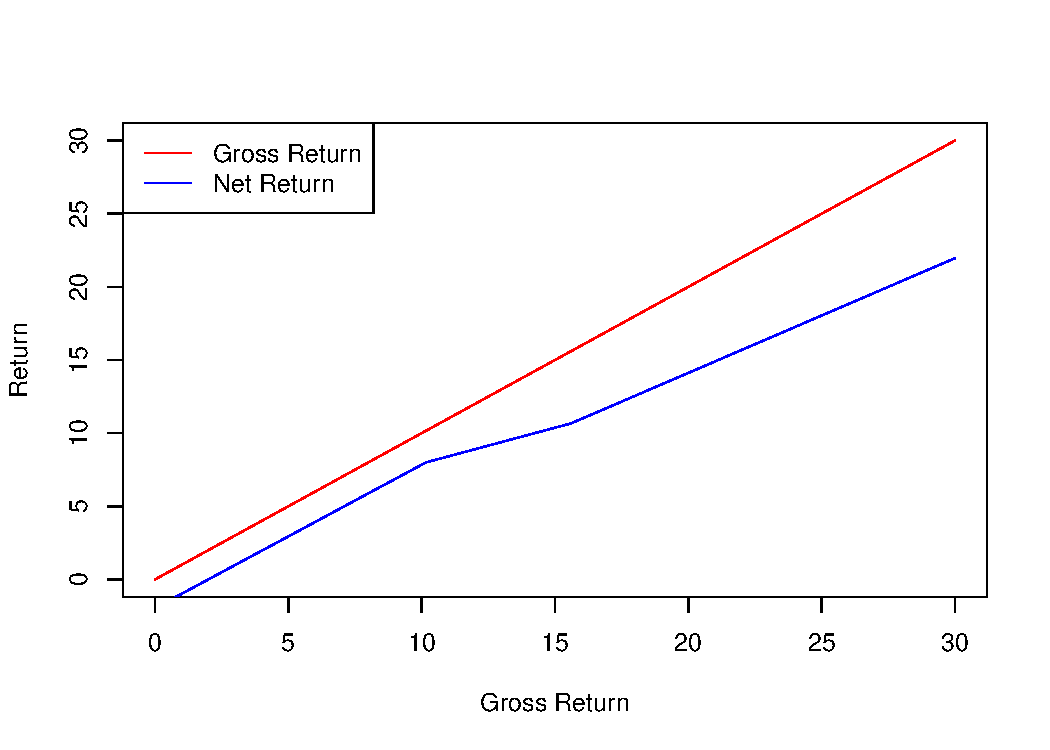
\includegraphics[width=\maxwidth]{figure/pe6-1} 

\end{knitrout}
\caption{General Partner Fee as Function of Gross Return}
%
\end{minipage}\hfill{}%
\begin{minipage}[t]{0.45\columnwidth}%
\begin{knitrout}
\definecolor{shadecolor}{rgb}{0.969, 0.969, 0.969}\color{fgcolor}
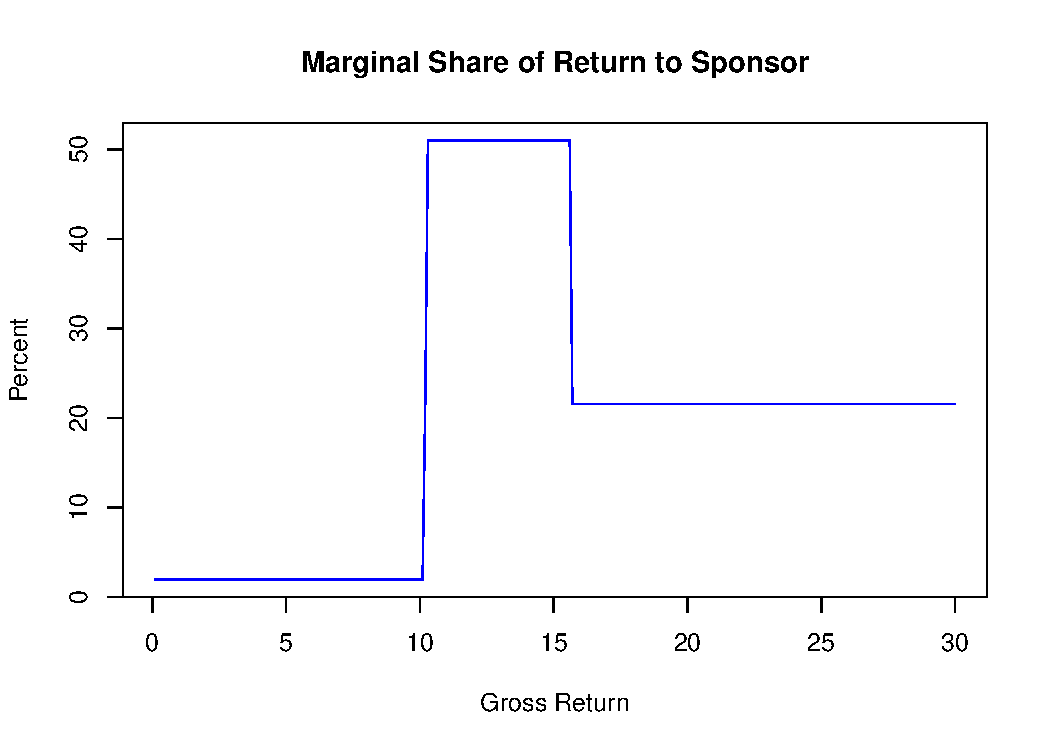
\includegraphics[width=\maxwidth]{figure/pe7-1} 

\end{knitrout}

\caption{Marginal Share of Return to Sponsor}
%
\end{minipage}
\end{figure}

Real estate deals have greater variation. Many real estate deals have
multiple layers, but no catchup. So, a real estate deal might be stated
as \textquotedbl 20 over 8, 30 over 12 and 50 over 20 with a 2\%
asset management fee, half of which is deferred until after 8\%\textquotedbl .
Stated this way, sponsor starts sharing 20\% of profits once the investor
earned an 8\% return, switching to 30\% of profits once the investor
has earned a 12\% return and 50\% of profits once the investor has
earned a 20\% return. Only 1\% of the asset management fee is paid
unconditionally. The remainder is paid once the investor has earned
8\%. Figure 3 shows the fee under this structure and figure 4 shows
the marginal share of earnings going to the sponsor at various gross
returns.



\begin{figure}[h]
\emph{Analysis of real estate structure ``20 over 8, 30 over 12,
50 over 20 with half of asset management deferred until after 8''}

\begin{minipage}[t]{0.45\columnwidth}%
\begin{knitrout}
\definecolor{shadecolor}{rgb}{0.969, 0.969, 0.969}\color{fgcolor}
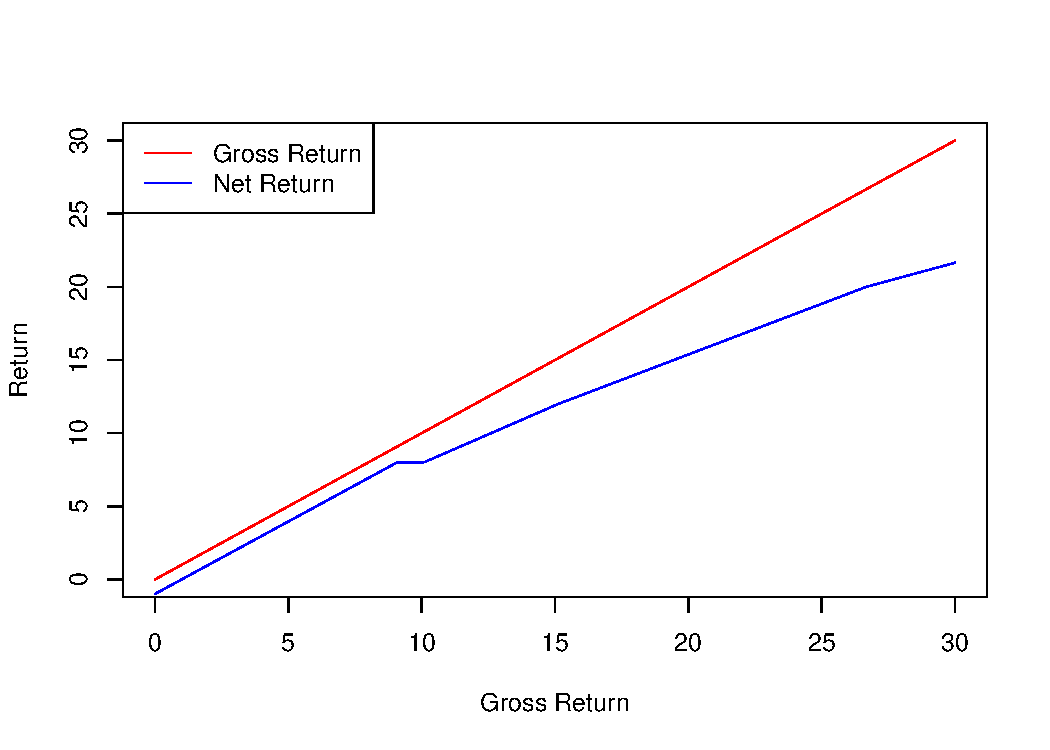
\includegraphics[width=\maxwidth]{figure/pe9-1} 

\end{knitrout}

\caption{Fees as Function of Gross Return}
%
\end{minipage}\hfill{}%
\begin{minipage}[t]{0.45\columnwidth}%
\begin{knitrout}
\definecolor{shadecolor}{rgb}{0.969, 0.969, 0.969}\color{fgcolor}
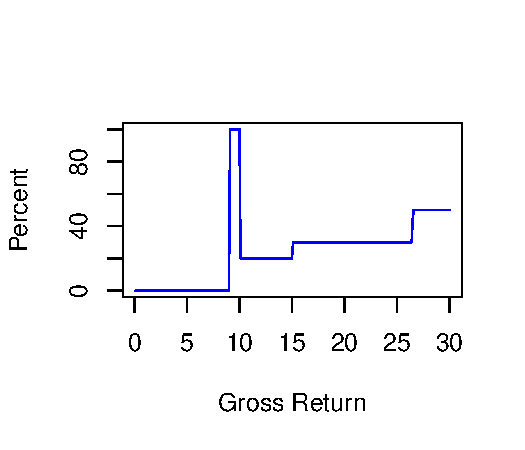
\includegraphics[width=\maxwidth]{figure/pe10-1} 

\end{knitrout}

\caption{Marginal Share of Return to Sponsor}
%
\end{minipage}
\end{figure}


\subsection*{Fee Effectiveness}

As part of evaluating an investment program, you will inevitably be
asked ``did you receive value for the fees you paid?'' I think the
best way to look at this is by considering fees as a percent of excess
profits. Let's revisit the real estate example structure and suppose
that we consider 6\% to be a reasonable hurdle rate for real estate.
Figure 5 shows the fees paid under that structure as a percent of
excess return.

\begin{figure}
\emph{Further Analysis of the ``20 over 8, 30 over 12, 50 over 20
with half of asset management deferred until after 8'' structure}

\begin{minipage}[t]{0.45\columnwidth}%


\begin{knitrout}
\definecolor{shadecolor}{rgb}{0.969, 0.969, 0.969}\color{fgcolor}
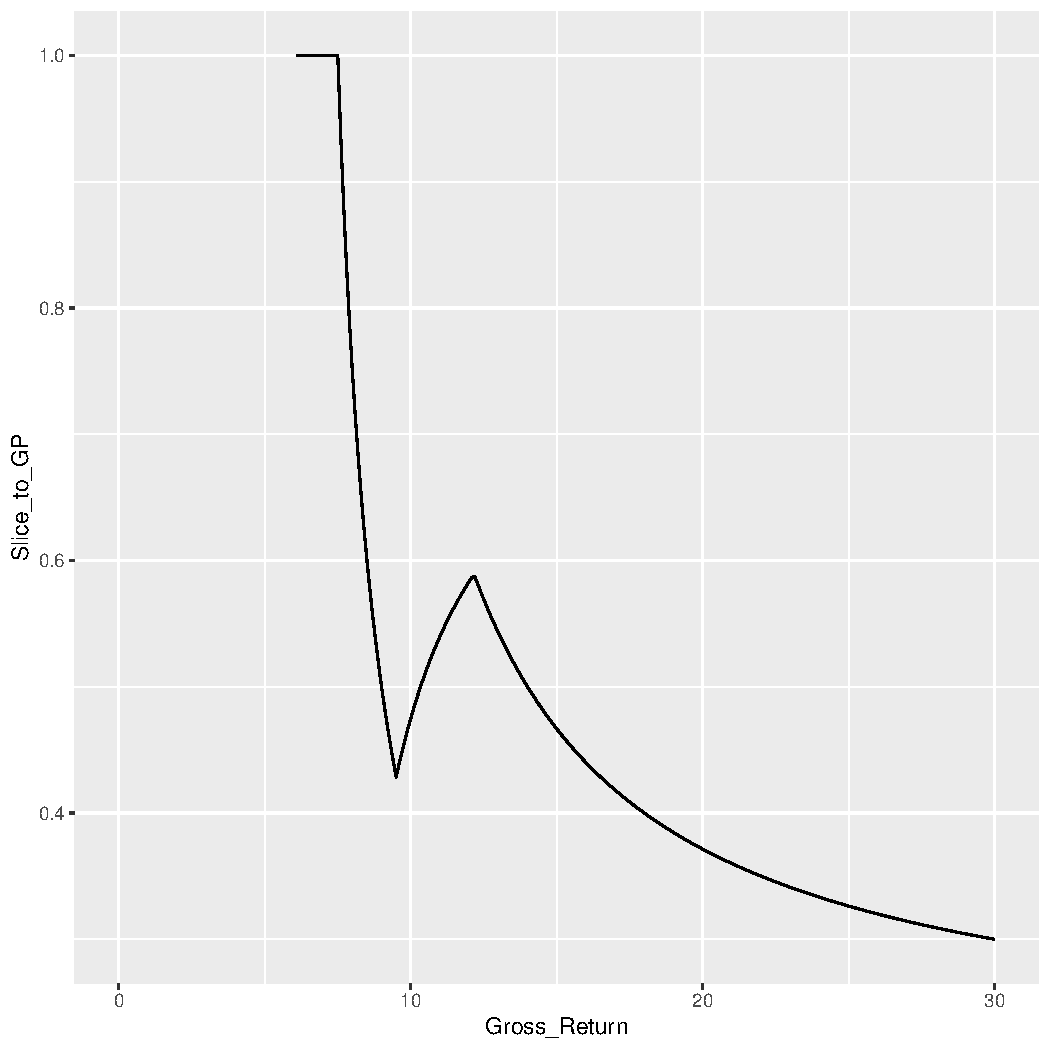
\includegraphics[width=\maxwidth]{figure/ce3-1} 

\end{knitrout}

\caption{Fee Effectiveness}
%
\end{minipage}\hfill{}%
\begin{minipage}[t]{0.45\columnwidth}%
\begin{knitrout}
\definecolor{shadecolor}{rgb}{0.969, 0.969, 0.969}\color{fgcolor}
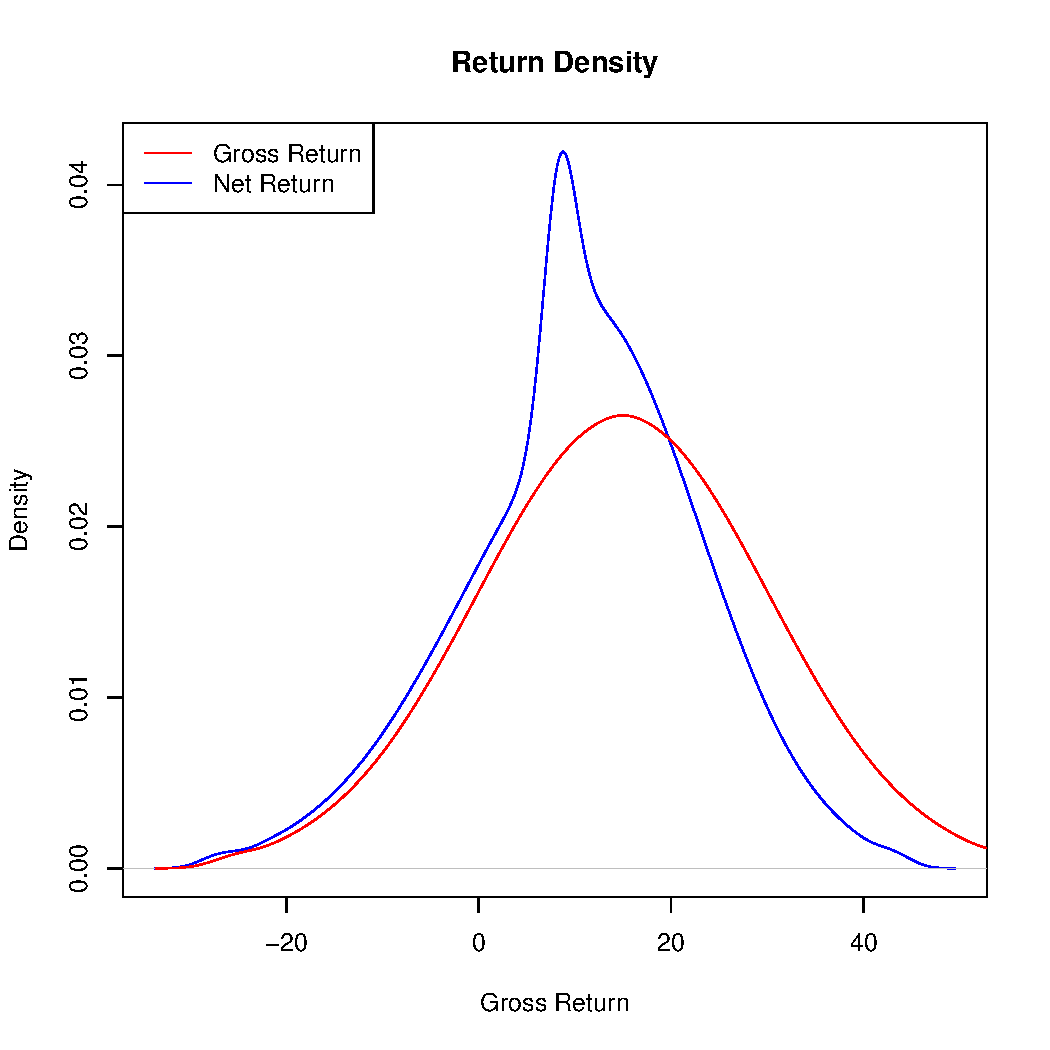
\includegraphics[width=\maxwidth]{figure/skew2-1} 

\end{knitrout}

\caption{Skewness of Net Returns}
%
\end{minipage}
\end{figure}


\subsection*{Consideration of skewness}

Investment results are skewed by these compensation structures. Investors
own all of the downside but share the upside with the sponsor. Suppose
we think for a particular investment gross returns are normally distributed,
with a mean of 15\% and standard deviation of 15\%. How are the net
returns distributed? Figure 6 shows the skewness of net returns using
the multi-tier real estate structure described previously.

\subsection*{Negotiating terms to manage cost}

The primary fee cost drivers in private equity type investment are
the asset management and incentive fees. If you are trying to negotiate
and reduce cost, here are some suggestions on where to direct your
focus.

Pay close attention to the catch-up provisions. Assuming your incentive
fee is 20 over 8 and a reasonably successful investment program, the
catchup will add 1.6\% per year to the investment cost; i.e. the 20\%
incentive rate times the 8\% hurdle. While this would be considered
market standard in many contexts, it may at times be negotiable. The
catchup has the biggest impact in the return band of 9\% to 12\% gross
returns, where the catchup is paid. If this is an interemediate return
strategy (as many real estate and credit strategies will be) where
the expected returns are within that band, you need to consider whether
this is acceptable to you. Negotiated solutions might be elimination
of the catchup, possibly in consideration for a lower hurdle or the
addition of higher incentive structures for exceptional performance
as in the real estate structure described above.

Asset management fees are charged on either ``committed'' or ``invested''
capital. In the former case you pay a fee on the full amount of capital
committed whether or not it has been called. Assuming investments
are made ratably over the first three years of the partnership, this
adds 1.5 times the annual fee rate over the life of the fund. Assuming
an annual fee rate of 1.5\% and weighted average duration of investments
of eight years, the annual additional cost is a little less then 30bp
per year. This is a fraction of the cost of the catchup, but still
important. You need to keep in mind the big picture. If your manager
is smaller, they may need the early revenue to support a proper team
for your strategy and you might better serve yourself by focusing
on other areas for cost savings. But compromises may be available
in the form of reduced fees on committed capital or performance based
fees that link fees to achieved operational results.

Finally, you should pay careful attention to what services are funded
by the asset management fees and what services are charged as additional
fund expenses to the partnership or charged to the deals. Read the
manager's ``ADV'' forms filed with the SEC. There is a lot of useful
disclosure here. 

\subsection*{When Alignment of Interest Fails}

By sharing profits with an asset manager, you achieve alignment of
interest with them. At least while things are going well. The system
falls apart with underperforming investments. With underperforming
investments there is no incentive for the manager to wrap up the partnership.
In fact, the manager is better off avoiding asset sales to continue
the asset management fees and for the option value on the incentive
fee in case the asset recovers. The investor may well prefer to sell
and recover their capital from an underperforming investment in order
to move on to the next thing.

The situation is exacerbated when incentive fees are paid on a deal
by deal basis. In that case if the manager has sold profitable deals
early in the partnership and collected incentive fees for them, they
may owe the partnership money for a ``clawback'' on liquidation
of the partnership. This arises when fees initially advanced for early
deals are higher than ultimately earned on the partnership as a whole.
This provides a powerful additional incentive to delay final liquidation.

For an investor in a program constructed of traditional closed end
fund partnership interests there is little defense against these problems
other than a well diversified portfolio with multiple managers, strategies
and vintages. In that portfolio structure any problems will be mitigated
and you can gradually weed out any managers who handle tough situations
poorly.

However, if you are a larger investor you may be able to structure
investments as large ``separate accounts'' on custom terms. In those
structures, you may be able to negotiate provisions in favor of the
investor for discretionary termination of investment periods, custom
mandatory investment criteria and ability to direct liquidation of
all or part of the assets. This approach is much more management intensive
and requires specialized expertise to implement, but can add significant
value in reduced cost and reliably aligned interests.

One cautionary remark on larger alternate investment structures is
that just being larger and just reducing fees isn't enough to produce
better results. A number of larger investors have pursued ``co-invest
sidecar'' structures where they get investment allocations side by
side with a traditional investment fund at reduced or no fees. The
criteria for investment allocation vary, but generally larger deals
are allocated partly to the co-invest vehicles. Josh Lerner and Antoinette
Schoar analyzed a large database of investments in these types of
alternate vehicles and concluded that the alternate structures underperformed
the related fund investments for many investors \parencite{Lerner2018}.
If you are going to pursue alternate and larger structures you will
need to mitigate the risk of increased concentration through an appropriate
partnership structure with adequate rights to ensure strategy discipline
and liquidity rights. Just pursuing a larger relationship in order
to negotiate lower fees may not add value.

\subsection*{Information rights}

An area of ongoing frustration for me has been the quality and timeliness
of information delivered to investors. Investors often receive information
which is partial, not consistently presented from quarter to quarter
and heavily spun by the firm's marketing department. Investors should
have access to real financial statements for each of the portfolio
investments, prepared in accordance with GAAP consistently applied
and delivered promptly. Additionally, there should be management discussion
including a set of key performance indicators relevant to the deal
and compared to initial underwriting expectations. With this information,
an investor could know if an investment is going well.

\section*{THE UPSHOT}

When I started to write this paper, I thought it was going to be about
the quantitative methods. I've written code which I believe could
be a minor, but useful addition to the field and made it available
on a github repository. It quickly dawned on me that this would create
the wrong impression, as though implementing these quantitative tricks
would lead to a successful investment program. So, I changed the focus
to describe the decision process that the quantitative methods are
serving.

The most important determinant of investment success are strategy
selection and investment manager hiring decisions. Private markets
investing is business investing. Viable strategies exist in every
industry and may be growth or value oriented. It's incumbent on the
investor to consider the business propositions carefully and assess
whether they add value and create strategic advantage in addressing
a viable market.

Manager hiring decisions are key to successfully implementing the
strategies you have selected. You need to assess the fit of the organization
to the strategy -- the organization needs depth and expertise in
the industries, products and managerial disciplines needed by the
strategy. The organization needs to be healthy with a strong and motivated
team. The PME methods discussed here provide a rigorous way to assess
whether a manager has in fact added value. But that measurement is
only useful in support of your assessment that an organization is
well suited to implement a strategy you have chosen to pursue. If
you flip the order and conclude something like ``the PME was good,
the strategy and the firm must be good'', you are (in my opinion)
making a mistake.

Negotiation of terms matters. The best way to think about cost is
as a percent of excess return and we have presented methods for analyzing
and understanding cost. Minimization of cost is not the goal. Indeed,
if you are successful in selecting high performing strategies and
management teams your absolute cost will be higher because you will
pay more in incentive fees. You need to negotiate fees keeping in
mind the big picture -- you want to encourage and support your partners
to build and maintain high quality teams and the fees paid need to
be consistent with that. The mix and timing of fees paid needs to
be logical for the firm you have chosen as your partner. But when
the dust settles, you want the fees to bear a reasonable relationship
to excess returns earned. As the investor you are taking essentially
all of the risk and need to retain a fair share of the reward.

How has this worked out for ASRS? During the ten years I've worked
at ASRS, it has built a private markets program consisting of real
estate, private equity and credit that now amounts to about 40\% of
its fund value and is targeted to be about 50\% of the fund in coming
years. Over that ten year period, the private markets investments
have exceeded their benchmarks with annual excess returns for the
ten year period of 1.7\% for private equity, 2.7\% for real estate
and 5.1\% for credit. In the most recent year ended June 30, 2019,
the excess returns were 7.5\% for private equity, 3.7\% for real estate
and 2.3\% for credit\footnote{The benchmarks are ODCE for real estate, Russell 2000 for private
equity and the LSTA leveraged loan index + 250bp for credit.}. ASRS has made extensive use of large separate accounts and some
direct investments in implementing its real estate and credit program.
These alternate structures have outperformed commingled fund vehicles
and provide the additional benefit of much closer market engagement
providing opportunity for building greater expertise and honing of
skills. These excess returns have added over \$2 billion of value
to the ASRS trust fund and contributed to the overall performance
of ASRS which has placed it consistenly among the top quartile of
public pension plans. \footnote{Detailed information about ASRS investment performance is found in
reports to the board investment committee and posted on the ASRS website
at \href{http://azasrs.gov/content/board-and-committee-meetings}{azasrs.gov/content/board-and-committee-meetings}}

I'd like to close with some thoughts about research and potential
reform. In the research area, the quantitative research and introduction
of techniques (notably PME) is useful. But more organizational oriented
research would help. Are there characteristics of firms (such as growth,
sharing of carry, management of careers) that can be associated with
higher likelihood of success? On the industry side, the near universality
of ``20 over 8'' as an incentive structure should be questioned.
Fund sponsors rightly point out that the 8\% hurdle may not be appropriate
in a 2\% treasury world. Incentive compensation linked to excess return
relative to market indices may be an improvement and use of PME methods
in measuring excess performance appropriate. Reform is needed to improve
alignment on underperforming funds. The languishing of out-of-the-money
funds is common and creates the appearance they are being exploited
for fees. Investors need remedies and structures to address this.
Finally, progress in the quality and timeliness of information delivered
to investors would be a great boon to them.

Thank you for reading this article! I hope you found it useful.

\printbibliography

\end{document}
